\section{Path from C to Assembly}
\begin{frame}{Target Lowering Steps}
    \begin{tikzpicture}[node distance = 2cm, auto]
\centering
\tikzstyle{every node}=[font=\footnotesize]
    % Place nodes
    \node [block] (init) {C code};
    \node [cloud, left of=init,node distance=2.5cm] (ast) {Clang AST};
    \node [block, left of=ast,node distance=2.5cm] (llvmir) {LLVM IR};
    \node [cloud, below of=llvmir,node distance=2.5cm] (opt1) {Optimize};
    \node [cloud, right of=opt1,node distance=2.5cm] (leg) {Legalize};
    \node [cloud, right of=leg,node distance=2.5cm] (opt2) {Optimize};
    \node [cloud, right of=opt2,node distance=2.5cm] (sel) {Instr. Selection};
    \node [cloud, right of=opt2,node distance=2.5cm] (sched) {Instr. Scheduling};
    \node [cloud, below of=sel,node distance=2.5cm] (reg) {Register Allocation};
    \node [block, left of=reg,node distance=2.5cm] (assem) {Assembly};

    % Draw edges
    \path [line] (init) -- (ast);
    \path [line] (ast) -- (llvmir);
    \path [line] (llvmir) -- (opt1);
    \path [line] (opt1) -- (leg);
    \path [line] (leg) -- (opt2);
    \path [line] (opt2) -- (sel);
    \path [line] (sel) -- (sched);
    \path [line] (sched) -- (reg);
    \path [line] (reg) -- (assem);
   
\end{tikzpicture}
\end{frame}

\begin{frame}[fragile]{Example C Code}
\begin{lstlisting}[language=C]
int a,b,c;
void maddFunc() {
	a = 3;
	b = 103;
	c = 127;
	a = a * b + c;
}
\end{lstlisting}
\end{frame}

\begin{frame}[fragile]{LLVM IR}
\lstinputlisting[caption={LLVM IR generated by Clang},label={fig:llvm_ir}, language=llvm, style=nasm]{../thesis/path_instruction/madd.ll}
\end{frame}


\begin{frame}{DAG After Legalization and Optimizations}
    \begin{figure}
    \centering
    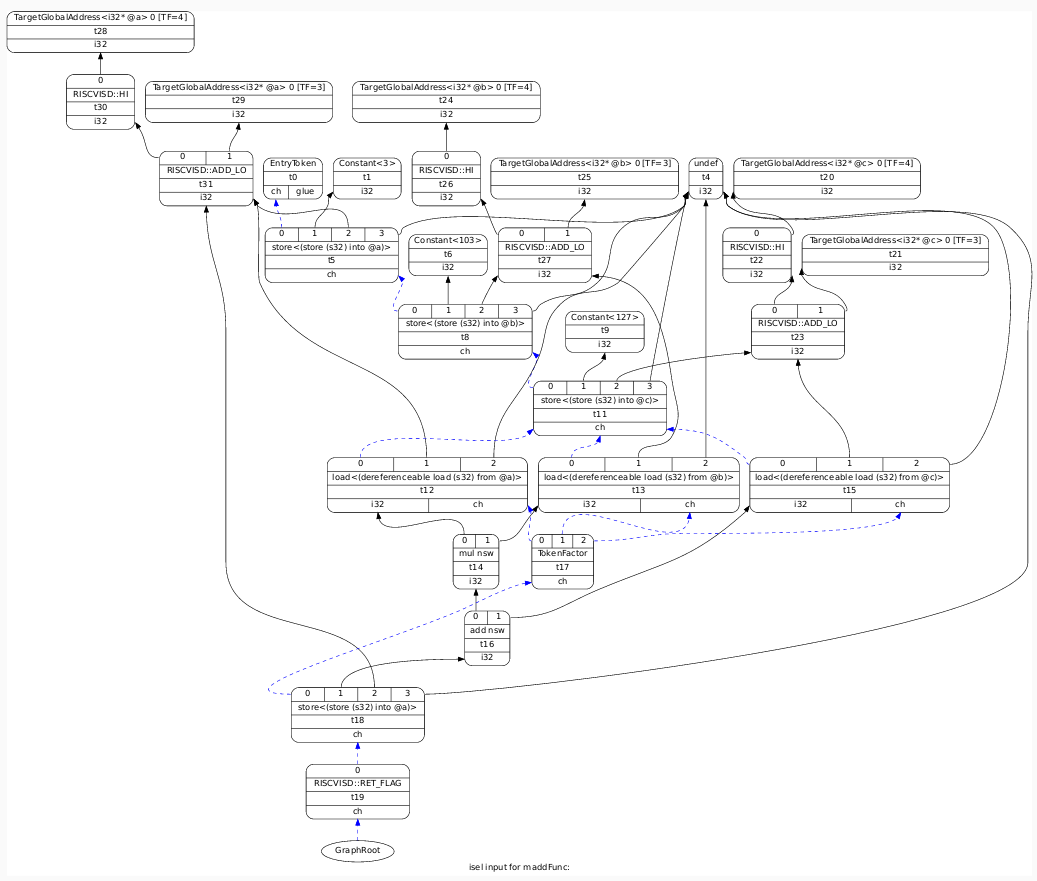
\includegraphics[height=0.75\textheight]{path_instruction/madd_dag_isel.png}
    \caption{DAG before Instruction Selection}
    \label{fig:isel}
\end{figure}
\end{frame}

\begin{frame}{DAG After Instruction Selection}
    \begin{figure}
    \centering
    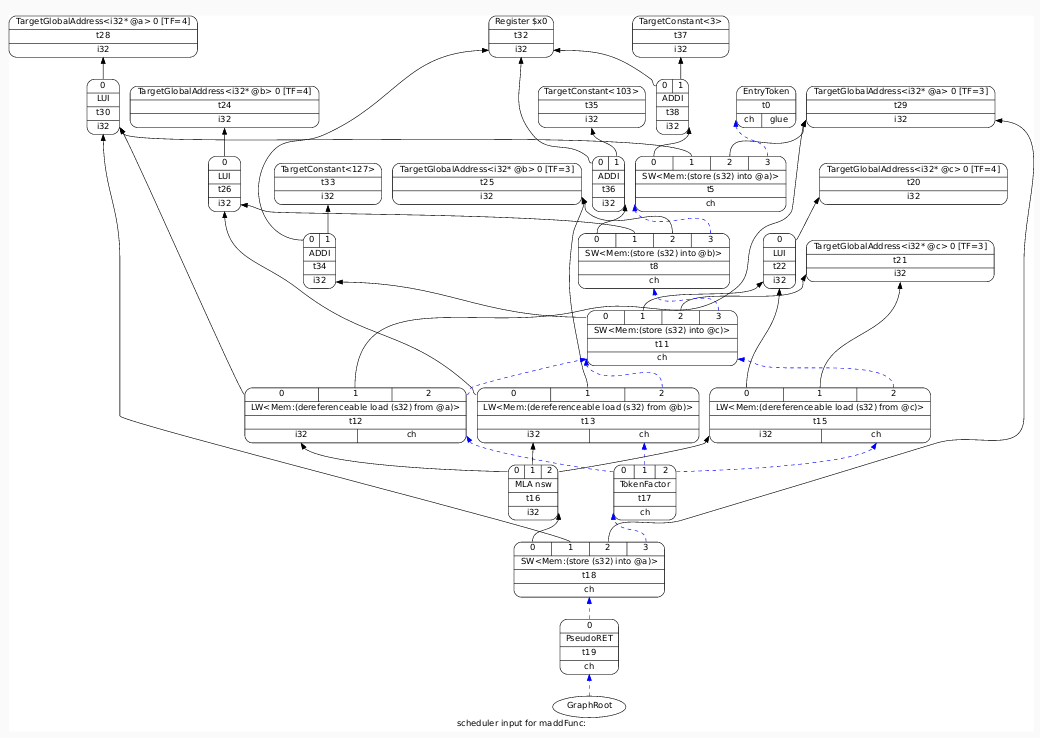
\includegraphics[height=0.75\textheight]{path_instruction/madd_dag_sched.png}
    \caption{DAG after Instruction Selection}
    \label{fig:dag_sched}
\end{figure}
\end{frame}


\begin{frame}[fragile]{Final Assembly}
    \begin{lstlisting}[ caption=madd.s Assembly Output]
    ...
	lui	a0, %hi(a)
	li	a1, 3
	sw	a1, %lo(a)(a0)
	lui	a1, %hi(b)
	li	a2, 103
	sw	a2, %lo(b)(a1)
	lui	a2, %hi(c)
	li	a3, 127
	sw	a3, %lo(c)(a2)
	lw	a3, %lo(a)(a0)
	lw	a1, %lo(b)(a1)
	lw	a2, %lo(c)(a2)
	mla	a1, a3, a1 ,a2
	sw	a1, %lo(a)(a0)
	lw	ra, 12(sp)     
	lw	s0, 8(sp)      
    ...
	ret
\end{lstlisting}
\end{frame}
